\scanpage{109}
\deleted{\unsure{be|have}} \inserted{one has} $M(r)\leq e^{(r^\sigma)}$ for $r$ sufficiently large.

\margin{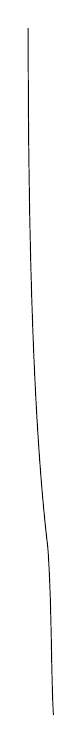
\begin{tikzpicture}[x=0.1mm,y=0.1mm,baseline=(current bounding box.north)]
\draw[line width=0.35pt] (0,0) .. controls (0,-260) and (6,-500) .. (25,-660) .. controls (30,-730) and (29,-815) .. (32,-872);
\end{tikzpicture}}
\uline{Theorem 2} (Hadamard-Borel) If the order $\rho$ of $f(z)$
is finite, then for \deleted{every} $\varepsilon>0$, the series
\[
\sum{}'\frac{1}{|a_n|^{\rho+\varepsilon}}<+\infty \tag*{(5)}
\]
($'$ indicates
that one does not sum over the zero roots)

Moreover, one then has (assuming $f(0)\ne0$)
\[
f(z)=e^{P(z)}\prod_n\left(1-\frac{z}{a_n}\right)e^{\frac{z}{a_n}+\mathord{-}+\frac{z^p}{p a_n^p}}
\]
where $p\leq\rho$, and $P(z)$ is \deleted{\unsure{a polynomial}} \inserted{a polynomial}
of degree $\leq\rho$ : in other words, one
has \qquad genus of $f$ $\leq\rho=$ order of $f$

\uline{Corollary} \quad If $\rho<1$, i.e if there exists a $0<\mu<1$
such that $M(r)\leq e^{(r^\mu)}$ for $r$ sufficiently large,
then $f(z)$ is of genus zero :
\[
f(z)=\mathrm{c}^{\mathrm{te}}\mathbin{\times}\prod_n\left(1-\frac{z}{a_n}\right)\deleted{\unsure{e^{z/a_n}}}
\]

\uline{Remark}. \quad It is very easy to convince oneself
that \qquad order of $f$ $\leq$ genus of $f+1$. Thus, if $\omega$ and
$g$ are respectively the genus and the order, one has
\begin{center}
\makebox[0pt][l]{\raisebox{-2mm}{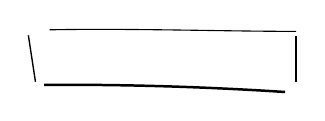
\begin{tikzpicture}[x=1mm,y=1mm]
\draw[line width=0.4pt] (2.7,7.2) .. controls (13,7.4) and (25,7.0) .. (34,7.0);
\draw[line width=0.5pt] (0,6.5) -- (0.9,0.6);
\draw[line width=0.45pt] (34,6.4) -- (34,0.6);
\draw[line width=0.9pt] (2,0.2) .. controls (14,0.3) and (25,-0.2) .. (32.6,-0.7);
\end{tikzpicture}}}\makebox[34mm]{\(\omega-1\leq g\leq\omega\)}
\end{center}

Since $\gamma$ is an integer, it follows that $\gamma$
is known as soon as $\omega$ is, unless $\omega$ is
an integer. In this case, one can have $p=\omega$, or
$\gamma=\omega-1$
\margin{110}
